\documentclass[c]{beamer}

%% Packages
\usepackage[utf8]{inputenc}
\usepackage[T1]{fontenc}
\usepackage[scaled=0.6]{DejaVuSansMono}
\usepackage[scaled=0.8]{DejaVuSans}
\usepackage{listings}
\usepackage{xcolor}
\usepackage{graphics}

%% Customize 'beamer'
\usetheme{PaloAlto}
\usecolortheme{dove}
\usefonttheme{professionalfonts}
\beamertemplatenavigationsymbolsempty
\logo{
\includegraphics[height=0.5cm]{/Users/scribb201/Pictures/comcast-nbcu.png}}

%% Solarized colors, stolen from https://github.com/jrnold/beamercolorthemesolarized
\definecolor{solarizedBase03}{HTML}{002B36}
\definecolor{solarizedBase02}{HTML}{073642}
\definecolor{solarizedBase01}{HTML}{586e75}
\definecolor{solarizedBase00}{HTML}{657b83}
\definecolor{solarizedBase0}{HTML}{839496}
\definecolor{solarizedBase1}{HTML}{93a1a1}
\definecolor{solarizedBase2}{HTML}{EEE8D5}
\definecolor{solarizedBase3}{HTML}{FDF6E3}
\definecolor{solarizedYellow}{HTML}{B58900}
\definecolor{solarizedOrange}{HTML}{CB4B16}
\definecolor{solarizedRed}{HTML}{DC322F}
\definecolor{solarizedMagenta}{HTML}{D33682}
\definecolor{solarizedViolet}{HTML}{6C71C4}
\definecolor{solarizedBlue}{HTML}{268BD2}
\definecolor{solarizedCyan}{HTML}{2AA198}
\definecolor{solarizedGreen}{HTML}{859900}
%% "Light" variant
\colorlet{solarizedRebase03}{solarizedBase3}
\colorlet{solarizedRebase02}{solarizedBase2}
\colorlet{solarizedRebase01}{solarizedBase1}
\colorlet{solarizedRebase00}{solarizedBase0}
\colorlet{solarizedRebase0}{solarizedBase00}
\colorlet{solarizedRebase1}{solarizedBase01}
\colorlet{solarizedRebase2}{solarizedBase02}
\colorlet{solarizedRebase3}{solarizedBase03}

%% Customize 'listings'
%% This isn't strictly necessary, but removes braces from the keywords
%% list. I'd really love to be able to control how identifiers are
%% printed, but it doesn't have full font-lock-like highlighting.
\lstdefinelanguage{Erlang}{
  morekeywords={after,begin,catch,case,cond,end,fun,if,let,of,receive,try,when,
    and,andalso,band,bnot,bor,bsl,bxor,div,not,or,orelse,rem,xor},
  otherkeywords={->,!,<-,<=},%
  sensitive=true,
  morecomment=[l]\%,
  morestring=[b]",
  morestring=[b]'
  }

%% Use the solarized colors for listings
\lstset{language=Erlang,
  backgroundcolor=\color{solarizedRebase03},
  basicstyle=\small\color{solarizedRebase0}\ttfamily,
  keywordstyle=\bfseries\color{solarizedGreen},
  identifierstyle=\color{solarizedBlue},
  commentstyle=\color{solarizedRebase01}\itshape,
  stringstyle=\color{solarizedCyan},
  showstringspaces=false,
  frame=single,frameround=tttt,framesep=0.6em,
  emphstyle=\bfseries\color{solarizedRed}}

\title[EUC 2015]{Techniques for Metaprogramming in Erlang}
%% \subtitle{\textit{Code Generation is Your Friend!}}
\author[Sean Cribbs]{\Large Sean Cribbs \\
  \small{Comcast Cable (T+PD) \\ @seancribbs}}
\date[EUC 2015]{Erlang User Conference \\ Stockholm \\
  12 June 2015}


\begin{document}

\begin{frame}
  \maketitle
\end{frame}

\begin{frame}{About me}
  \begin{itemize}
  \item \textbf{Senior Principal Engineer} at Comcast Cable
  \item Former \textbf{Technical Lead} for Riak at Basho
  \item Creator of \texttt{neotoma}, Erlang \textbf{packrat-parser toolkit}
  \end{itemize}
\end{frame}

\section{Background}

\begin{frame}[c]
  \begin{center}
    \Huge Background
  \end{center}
\end{frame}

\begin{frame}{What is Metaprogramming?}
  \begin{columns}[t]
    \column{0.45\textwidth}
      \begin{itemize}
      \item Code writing code
      \item Programs as data
        \begin{itemize}
        \item Reflection / reflexivity
        \item Homoiconicity
        \end{itemize}
      \end{itemize}
    \pause
    \column{0.45\textwidth}
      \begin{itemize}
      \item Run-time\pause
      \item \textbf{Compile-time}
      \end{itemize}
  \end{columns}
\end{frame}

\begin{frame}{Why Metaprogram?}
  \begin{itemize}
  \item Reduce duplication
  \item Inject optimization
  \item Simplify APIs
  \item Improve tools
  \item Implement DSLs
  \end{itemize}
\end{frame}

\begin{frame}[c]{Metaprogramming Erlang}
  \begin{center}
    \includegraphics[height=\textheight]{steps.pdf}
  \end{center}
\end{frame}

%%----------------------------------------------------
\section{Macros}

\begin{frame}[c]
  \begin{center}
    \Huge Technique 1 \\ Macros
  \end{center}
\end{frame}

\begin{frame}[fragile,t]{Macros}
  \begin{itemize}
  \item Generates code in preprocessor (\texttt{epp})
  \item Operates over \textbf{Tokens} (mostly)
  \end{itemize}
  \begin{onlyenv}<1>
    \begin{lstlisting}
% static term
-define(TIMEOUT, 5000).
\end{lstlisting}
  \end{onlyenv}

  \begin{onlyenv}<2>
    \begin{lstlisting}
% static term
-define(TIMEOUT, 5000).
% parameterized
-define(THUNK(A), fun() -> (A) end).
-define(IF(B,T,F),
        begin
        (case (B) of true->(T); false->(F) end)
        end).
\end{lstlisting}
  \end{onlyenv}

  \begin{onlyenv}<3>
    \begin{lstlisting}
% static term
-define(TIMEOUT, 5000).
% parameterized
-define(THUNK(A), fun() -> (A) end).
-define(IF(B,T,F),
        begin
        (case (B) of true->(T); false->(F) end)
        end).
%% escaped arguments
-define(Quote(A), io_lib:format("~s",[??A])).
\end{lstlisting}
  \end{onlyenv}
\end{frame}

\begin{frame}[fragile]{Using Macros}
  \begin{lstlisting}
gen_server:call(?MODULE, ping, ?TIMEOUT).
%% gen_server:call(mymodule, ping, 5000).
  \end{lstlisting}
  \pause
  \begin{lstlisting}
Nope = ?THUNK(launch(missiles)).
%% Nope = fun() -> (launch(missiles)) end.
  \end{lstlisting}
  \pause
  \begin{lstlisting}
io:format("The value of ~s is ~p.", [?Quote(Foo), Foo]).
%% io:format("The value of ~s is ~p.",["Foo", Foo]).
  \end{lstlisting}
\end{frame}

\subsection{eunit}
\begin{frame}[fragile,t]{Macros - \texttt{eunit}}

  \begin{onlyenv}<1>
  \begin{lstlisting}
-define(assert(BoolExpr),
        begin
        ((fun () ->










            end
          end)())
        end).
  \end{lstlisting}
  \end{onlyenv}


  \begin{onlyenv}<2>
  \begin{lstlisting}
-define(assert(BoolExpr),
        begin
        ((fun () ->
            case (BoolExpr) of
                true -> ok;








            end
          end)())
        end).
  \end{lstlisting}
  \end{onlyenv}


  \begin{onlyenv}<3>
  \begin{lstlisting}
-define(assert(BoolExpr),
        begin
        ((fun () ->
            case (BoolExpr) of
                true -> ok;
                __V -> erlang:error({assertion_failed,
                                     [{module, ?MODULE},
                                      {line, ?LINE},
                                      {expression, (??BoolExpr)},
                                      {expected, true},
                                      {value, case __V of false -> __V;
                                                  _ -> {not_a_boolean,__V}
                                              end}]})
            end
          end)())
        end).
  \end{lstlisting}
  \end{onlyenv}
\end{frame}

\begin{frame}[fragile]{Macros - \texttt{eunit}}
  \begin{lstlisting}
fizzbuzz_test() ->
    ?assert(fizz =:= fizzbuzz(3)),
    ?assert(buzz =:= fizzbuzz(5)),
    ?assert(fizzbuzz =:= fizzbuzz(15)),
    ?assert(10 =:= fizzbuzz(10)).
  \end{lstlisting}
\pause
  \begin{verbatim}
1> eunit:test(mymodule).
mymodule: fizzbuzz_test (module 'mymodule')...*failed*
in function mymodule:'-fizzbuzz_test/0-fun-3-'/0 (mymodule.erl, line 18)
**error:{assertion_failed,[{module,mymodule},
                   {line,18},
                   {expression,"10 =:= fizzbuzz ( 10 )"},
                   {expected,true},
                   {value,false}]}
  \end{verbatim}
\end{frame}

\begin{frame}{Macros - Summary}
  \begin{columns}[t]
    \column{.45\textwidth}
      {\Large\color{solarizedGreen} Pros:}
      \begin{itemize}
      \item Easy and familiar
      \item Inline with program
      \item Syntax draws attention
      \end{itemize}

    \column{.45\textwidth}
      \pause
      {\Large\color{solarizedRed} Cons:}
      \begin{itemize}
      \item Limited expressivity
      \item Appearance
      \end{itemize}
  \end{columns}
  \pause
  \vskip 2.5em
  {\Large\color{solarizedBlue} Good for:}
  \begin{itemize}
  \item Small API wrappers like in \texttt{eunit} or \texttt{eqc}
  \item Naming constants
  \item Compile-time feature-switching (OTP upgrades)
  \item Debugging statements
  \end{itemize}
\end{frame}

%%----------------------------------------------------
\section{Parse Transforms}

\begin{frame}[c]
  \begin{center}
    \Huge Technique 2 \\ Parse Transforms
  \end{center}
\end{frame}


\begin{frame}[fragile]{Parse Transforms}
  \begin{itemize}
  \item Generates or transforms code after parsing
  \item Operates over \textbf{Abstract Form} (AST)
  \end{itemize}

  \begin{lstlisting}
%% In your module:
-compile([{parse_transform, the_transform_module}]).

%% In the parse transform module:
parse_transform(Forms, _Options) ->
    %% 'Forms' is the AST. 'Options' are the compiler options.
    %% Traverse/modify 'Forms' and return it
    Forms.
  \end{lstlisting}
  \pause
\begin{verbatim}
$ erlc -P mymodule.erl
$ cat mymodule.P
\end{verbatim}
\end{frame}

\subsection{lager}
\begin{frame}[fragile,t]{Parse Transforms - \texttt{lager}}
  \framesubtitle{github.com/basho/lager}
  \begin{itemize}
  \item Rewrites calls to \texttt{lager:SYSLOG\_SEVERITY\_LEVEL}
  \item Injects producer-side filtering and call-site metadata
  \end{itemize}
  \begin{onlyenv}<1>
  \begin{lstlisting}
lager:warning("Resource threshold exceeded ~p:~p", [Used, Available]).











  \end{lstlisting}
  \end{onlyenv}

    \begin{onlyenv}<2>
  \begin{lstlisting}[emph={Used,Available,warning}]
lager:warning("Resource threshold exceeded ~p:~p", [Used, Available]).
%% Becomes equivalent of:
case {whereis(lager_event), lager_config:get(loglevel, {0, []})} of
    {undefined, _} -> {error, lager_not_running};
    {Pid, {Level, Traces}} when (Level band 16) /= 0 orelse Traces /= [] ->
         lager:do_log(warning,[{module, mymodule}, {function, myfunc},
                               {line, 5}, {pid, pid_to_list(self())},
                               {node, node()} | lager:md()],
                     "Resource threshold exceeded ~p:~p",
                     [Used, Available], Level, Traces, Pid);
     _ -> ok
end.
  \end{lstlisting}
  \end{onlyenv}
\end{frame}

\begin{frame}[fragile]{Parse Transforms - \texttt{lager}}
  \framesubtitle{Understanding the AST}
  \begin{lstlisting}
{ok, Bin} = file:read_file("lager_snippet.erl"),
{ok, Tokens, _} = erl_scan:string(unicode:characters_to_list(Bin)),
{ok, AST} = erl_parse:parse_exprs(Tokens),
AST.
  \end{lstlisting}
  \pause
  \begin{lstlisting}[basicstyle=\color{solarizedRebase0}\ttfamily]
[{'case',1,
     {tuple,1,
            [{call,1,{atom,1,whereis},[{atom,1,lager_event}]},
             {call,1,
                   {remote,1,{atom,1,lager_config},{atom,1,get}},
                   [{atom,1,loglevel},{tuple,1,[{integer,1,0},{nil,1}]}]}]},
     [{clause,2,
              [{tuple,2,[{atom,2,undefined},{var,2,'_'}]}],
              [],
              [{tuple,2,[{atom,2,error},{atom,2,lager_not_running}]}]},
      {clause,3,
              [{tuple,3,
                      [{var,3,'Pid'},
                       {tuple,3,[{var,3,'Level'},{var,3,'Traces'}]}]}],
              [[{op,3,'orelse',
                    {op,3,'/=',
                        {op,3,'band',{var,3,'Level'},{integer,3,16}},
                        {integer,3,0}},
                    {op,3,'/=',{var,3,'Traces'},{nil,3}}}]],
              [{call,4,
                     {remote,4,{atom,4,lager},{atom,4,do_log}},
                     [{atom,4,warning},
                      {cons,4,
                            {tuple,4,[{atom,4,module},{atom,4,...}]},
                            {cons,4,{tuple,4,[...]},{cons,5,...}}},
                      {string,7,"Resource threshold exceeded ~p:~p"},
                      {cons,8,{var,8,'Used'},{cons,8,{var,...},{...}}},
                      {var,8,'Level'},
                      {var,8,'Traces'},
                      {var,8,'Pid'}]}]},
      {clause,9,[{var,9,'_'}],[],[{atom,9,ok}]}]}]
  \end{lstlisting}
\end{frame}

\begin{frame}[fragile]{Parse Transforms - \texttt{lager}}
  \framesubtitle{\texttt{lager\_transform} module}
\begin{lstlisting}[emph={walk_ast,AST}]
parse_transform(AST, Options) ->
    TruncSize = proplists:get_value(lager_truncation_size, Options,
                                    ?DEFAULT_TRUNCATION),
    Enable = proplists:get_value(lager_print_records_flag, Options, true),
    put(print_records_flag, Enable),
    put(truncation_size, TruncSize),
    erlang:put(records, []),
    %% .app file should either be in the outdir, or the same dir
    %% as the source file
    guess_application(proplists:get_value(outdir, Options), hd(AST)),
    walk_ast([], AST).
\end{lstlisting}
\end{frame}

\begin{frame}[fragile]{Parse Transforms - \texttt{lager}}
\framesubtitle{Recursing through the AST}
  \begin{lstlisting}[emph={walk_clauses}]
walk_ast(Acc, [{function, Line, Name, Arity, Clauses}|T]) ->
    put(function, Name),
    walk_ast([{function, Line, Name, Arity,
                walk_clauses([], Clauses)}|Acc], T);
  \end{lstlisting}
  \pause
  \begin{lstlisting}[emph={walk_body}]
walk_clauses(Acc, []) ->
    lists:reverse(Acc);
walk_clauses(Acc, [{clause, Line, Arguments, Guards, Body}|T]) ->
    walk_clauses([{clause, Line, Arguments, Guards, walk_body([], Body)}|Acc], T).
  \end{lstlisting}
  \pause
  \begin{lstlisting}[emph={transform_statement}]
walk_body(Acc, []) ->
    lists:reverse(Acc);
walk_body(Acc, [H|T]) ->
    walk_body([transform_statement(H)|Acc], T).
  \end{lstlisting}
\end{frame}

\begin{frame}[fragile]{Parse Transforms - \texttt{lager}}
\framesubtitle{Transforming matching calls}
\begin{lstlisting}[emph={Severity,lager}]
transform_statement({call, Line, {remote, _Line1, {atom, _Line2, lager},
            {atom, _Line3, Severity}}, Arguments0} = Stmt) ->
    case lists:member(Severity, ?LEVELS) of
        false -> Stmt;   %% NB: Don't modify if it isn't a severity level!
        true -> %%...
    end;
\end{lstlisting}
\end{frame}

\begin{frame}[fragile]{Parse Transforms - \texttt{lager}}
\framesubtitle{Checking the logging conditions}
\begin{lstlisting}[emph={lager,do_log}]
LevelVar = make_varname("__Level", Line),
TracesVar = make_varname("__Traces", Line),
PidVar = make_varname("__Pid", Line),
%% case {whereis(lager_event),
%%       lager_config:get(loglevel,{?LOG_NONE, []})} of
{'case', Line,
   {tuple, Line,
       [{call, Line, {atom, Line, whereis}, [{atom, Line, lager_event}]},
        {call, Line, {remote, Line, {atom, Line, lager_config}, {atom,
              Line, get}},
          [{atom, Line, loglevel}, {tuple, Line, [{integer, Line, 0},
                                                  {nil, Line}]}]}]},
   [
     %% case clauses ...
   ]}
\end{lstlisting}
\end{frame}

\begin{frame}[fragile,t]{Parse Transforms - \texttt{lager}}
  \framesubtitle{The log dispatch clause}
    \begin{onlyenv}<1>
\begin{lstlisting}
{clause, Line,
    %% Match
    [{tuple, Line, [{var, Line, PidVar}, {tuple, Line, [{var, Line, LevelVar},
                                                        {var, Line,
                                                          TracesVar}]}]}],
    % ...
    %
    %
    %
    %
    %
    %
    %
    %
    %
    %
    %
\end{lstlisting}
  \end{onlyenv}
  \begin{onlyenv}<2>
\begin{lstlisting}
{clause, Line,
    %% Match
    [{tuple, Line, [{var, Line, PidVar}, {tuple, Line, [{var, Line, LevelVar},
                                                        {var, Line,
                                                          TracesVar}]}]}],
    %% Guards
    [[{op, Line, 'orelse',
          {op, Line, '/=', {op, Line, 'band', {var, Line, LevelVar},
                                              {integer, Line,
                                                SeverityAsInt}},
                           {integer, Line, 0}},
          {op, Line, '/=', {var, Line, TracesVar}, {nil, Line}}}]],
    % ...
    %
    %
    %
    %
\end{lstlisting}
  \end{onlyenv}
  \begin{onlyenv}<3>
\begin{lstlisting}
{clause, Line,
    %% Match
    [{tuple, Line, [{var, Line, PidVar}, {tuple, Line, [{var, Line, LevelVar},
                                                        {var, Line,
                                                          TracesVar}]}]}],
    %% Guards
    [[{op, Line, 'orelse',
          {op, Line, '/=', {op, Line, 'band', {var, Line, LevelVar},
                                              {integer, Line,
                                                SeverityAsInt}},
                           {integer, Line, 0}},
          {op, Line, '/=', {var, Line, TracesVar}, {nil, Line}}}]],
    %% Statements
    [
    %% do the call to lager:dispatch_log
    {call, Line, {remote, Line, {atom, Line, lager}, {atom, Line, do_log}},
        [             % ...
\end{lstlisting}
  \end{onlyenv}
\end{frame}

\subsection{parse\_trans}

\begin{frame}[c]{Parse Transforms - \texttt{parse\_trans}}
  \framesubtitle{github.com/uwiger/parse\_trans}
  \begin{columns}[c]
    \column{.45\textwidth}
    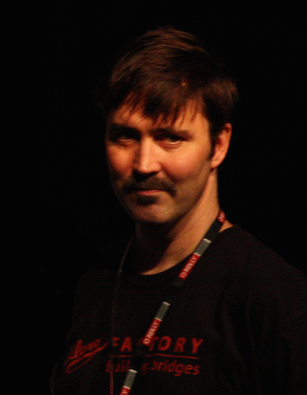
\includegraphics[width=\textwidth]{ulf_wiger.png}

    \column{.45\textwidth}
    Don't worry\ldots
    \par {\Large Ulf has your back!}
  \end{columns}
\end{frame}

\begin{frame}[fragile]{Parse Transforms - \texttt{parse\_trans}}
  \framesubtitle{Rewriting lager's transform with \texttt{parse\_trans}}
  \begin{itemize}
  \item Write transformations as ``visitors'' instead of manual recursion
  \item Return \texttt{NewForm} to replace the current form
  \item Return \texttt{continue} to recurse into subexpressions
  \end{itemize}

  \begin{lstlisting}
parse_transform(AST, Options) ->
    %% Previously: walk_ast([], AST)
    parse_trans:plain_transform(fun do_transform/1, AST).
  \end{lstlisting}
  \pause
  \begin{lstlisting}
do_transform({call, _Line, {remote, _Line1, {atom, _Line2, lager},
                            {atom, _Line3, _Severity}}, _Arguments0} = Stmt) ->
    %% Do what we did before...
    transform_statement(Stmt);
do_transform(_) ->
    continue.
  \end{lstlisting}
\end{frame}

\begin{frame}{Parse Transforms - \texttt{parse\_trans}}
  \framesubtitle{Other cool stuff!}
  \begin{itemize}
  \item \texttt{ct\_expand} - compile-time evaluation
  \item \texttt{exprecs} - generates record-accessor functions
  %% \item \texttt{parse\_trans\_codegen} - generates code via template
  %%   substitution
  %% \item \texttt{parse\_trans\_mod} - extract, rename, compile/load
  \end{itemize}
\end{frame}

\begin{frame}{Parse Transforms - Summary}
  \begin{columns}[t]
    \column{.45\textwidth}
      {\Large\color{solarizedGreen} Pros:}
      \begin{itemize}
      \item Powerful
      \item Erlang syntax
      \item Compile-time computation
      \end{itemize}

    \column{.45\textwidth}
      \pause
      {\Large\color{solarizedRed} Cons:}
      \begin{itemize}
      \item Hides ``magic''
      \item Difficult to write/debug
      \item Only modifies current module
      \end{itemize}
  \end{columns}
  \pause
  \vskip 2.5em
  {\Large\color{solarizedBlue} Good for:}
  \begin{itemize}
  \item Injecting optimizations or new semantics
  \item Embedded DSLs
  \item Generating code in same module
  \end{itemize}
\end{frame}


%%----------------------------------------------------
\section{Syntax Trees}

\begin{frame}[c]
  \begin{center}
    \Huge Technique 3 \\ Syntax Trees
  \end{center}
\end{frame}

\begin{frame}[fragile]{Syntax Trees}
  \begin{itemize}
  \item Generates code by constructing syntax trees
  \item Operates over \textbf{Abstract Forms}
  \end{itemize}
\end{frame}

\subsection{erl\_syntax}

\begin{frame}{Syntax Trees - \texttt{erl\_syntax}}
  \begin{itemize}
  \item Datatype for \textbf{Abstract forms}
  \item Functions for every construct
  \end{itemize}
  \begin{center}
    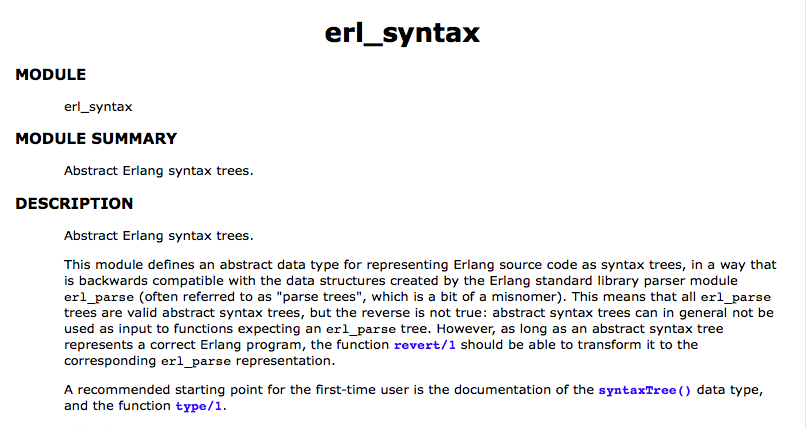
\includegraphics[width=\textwidth]{erl_syntax.png}
  \end{center}
\end{frame}

\begin{frame}{Syntax Trees - \texttt{erl\_syntax}}
  \begin{itemize}
  \item<1-> Creating nodes: \\
    \texttt{integer/1 float/1 atom/1 variable/1} \\
    \texttt{list/2 cons/2 tuple/1} \\
    \texttt{block\_expr/1 clause/2,3 fun\_expr/1} \\
    \texttt{conjunction/1 disjunction/1} \\
    \texttt{function/2 attribute/2 form\_list/1}
  \item<2-> Inspecting nodes: \\
    \texttt{type/1 float\_value/1 attribute\_name/1}
  \item<3-> Converting: \\
    \texttt{abstract/1 revert/1 revert\_forms/1}
  \item<4> Traversing: \texttt{subtrees/1}
  \end{itemize}
\end{frame}

\subsection{Neotoma}
\begin{frame}[c]{Syntax Trees - Neotoma v1}
  \framesubtitle{Getting out my shinebox}
  \begin{center}
      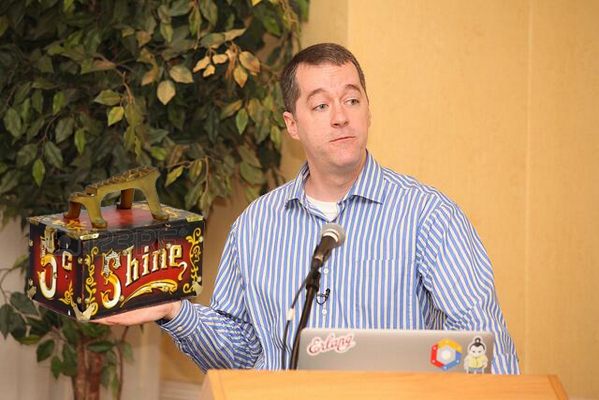
\includegraphics[width=\textwidth]{shinebox.png}
  \end{center}
\end{frame}

\begin{frame}[fragile,t]{Syntax Trees - Neotoma v1}
  \framesubtitle{github.com/seancribbs/neotoma}
  \begin{lstlisting}
quoted_string <- single_quoted_string / double_quoted_string
%{
  used_combinator(p_string),
  lists:flatten(["p_string(<<\"",
   escape_string(unicode:characters_to_list(proplists:get_value(string, Node))),
   "\">>)"])
%};
  \end{lstlisting}
  \pause
  \begin{lstlisting}
generate_module_attrs(ModName, Combinators) ->
    ["-module(", atom_to_list(ModName) ,").\n",
     "-export([parse/1,file/1]).\n",
     [ generate_combinator_macro(C) || Combinators /= undefined,
                                       C <- Combinators ],
     "\n"
     ].
  \end{lstlisting}

\end{frame}

\begin{frame}[fragile,t]{Syntax Trees - Neotoma v2}
  \begin{lstlisting}
quoted_string <- single_quoted_string / double_quoted_string
%{
  #string{string = unicode:characters_to_binary(proplists:get_value(string,
                                                                    Node)),
          index = Idx}
%};
  \end{lstlisting}
\end{frame}

\begin{frame}[fragile,t]{Syntax Trees - Neotoma v2}

    \begin{lstlisting}
case Input of
    <<"a string"/binary, Input1/binary>> -> % ...do the success path;
    _ -> % ...do the failure path
end
    \end{lstlisting}
    \pause
    \begin{onlyenv}<2>
  \begin{lstlisting}
generate(#string{string=S}, InputName, Success, Fail) ->
  \end{lstlisting}
    \end{onlyenv}

    \begin{onlyenv}<3>
  \begin{lstlisting}
generate(#string{string=S}, InputName, Success, Fail) ->
    Literal = abstract(S), % convert term to syntaxTree()
    RestName = variable(new_name("Input")),
  \end{lstlisting}
    \end{onlyenv}

    \begin{onlyenv}<4>
  \begin{lstlisting}
generate(#string{string=S}, InputName, Success, Fail) ->
    Literal = abstract(S),
    RestName = variable(new_name("Input")),
    case_expr(InputName, % case ... of ... end
  \end{lstlisting}
    \end{onlyenv}

    \begin{onlyenv}<5>
  \begin{lstlisting}
generate(#string{string=S}, InputName, Success, Fail) ->
    Literal = abstract(S),
    RestName = variable(new_name("Input")),
    case_expr(InputName,
              [clause([binary([binary_field(Literal, [atom("binary")]),
                               binary_field(RestName, [atom("binary")])])],
                      none,
                      Success(Literal, RestName)), % success path!
  \end{lstlisting}
    \end{onlyenv}
    \begin{onlyenv}<6>
  \begin{lstlisting}
generate(#string{string=S}, InputName, Success, Fail) ->
    Literal = abstract(S),
    RestName = variable(new_name("Input")),
    case_expr(InputName,
              [clause([binary([binary_field(Literal, [atom("binary")]),
                               binary_field(RestName, [atom("binary")])])],
                      none,
                      Success(Literal, RestName)),
               clause([underscore()], none,
                      Fail(InputName, error_reason({string, S})))]); % fail path!
  \end{lstlisting}
    \end{onlyenv}
\end{frame}

\subsection{mochiglobal}
\begin{frame}[fragile,t]{Syntax Trees - \texttt{mochiglobal}}
  \framesubtitle{github.com/mochi/mochiweb}
  \begin{itemize}
  \item Memoizes frequently used values in code
  \item Good for high-read, low-write scenarios
  \end{itemize}

  \begin{onlyenv}<1>
  \begin{lstlisting}
%% @doc Store term V at K, replaces an existing term if present.
put(K, V) ->
    put(K, V, key_to_module(K)).
  \end{lstlisting}
  \end{onlyenv}

  \begin{onlyenv}<2>
  \begin{lstlisting}
%% @doc Store term V at K, replaces an existing term if present.
put(K, V) ->
    put(K, V, key_to_module(K)).

put(_K, V, Mod) ->
    Bin = compile(Mod, V),
    code:purge(Mod),
    {module, Mod} = code:load_binary(Mod, atom_to_list(Mod) ++ ".erl", Bin),
    ok.
  \end{lstlisting}
  \end{onlyenv}
\end{frame}

\begin{frame}[fragile]{Syntax Trees - \texttt{mochiglobal}}

\begin{lstlisting}
-spec compile(atom(), any()) -> binary().
compile(Module, T) ->
    {ok, Module, Bin} = compile:forms(forms(Module, T),
                                      [verbose, report_errors]),
    Bin.
\end{lstlisting}
\pause
\begin{lstlisting}
forms(Module, T) ->
    [erl_syntax:revert(X) || X <- term_to_abstract(Module, term, T)].
\end{lstlisting}
\end{frame}

\begin{frame}[fragile,t]{Syntax Trees - \texttt{mochiglobal}}
  \begin{onlyenv}<1>
      \begin{lstlisting}
term_to_abstract(Module, Getter, T) ->
    [%% -module(Module).
     erl_syntax:attribute(
       erl_syntax:atom(module),
       [erl_syntax:atom(Module)]),
  \end{lstlisting}
  \end{onlyenv}

  \begin{onlyenv}<2>
      \begin{lstlisting}
term_to_abstract(Module, Getter, T) ->
    [%% -module(Module).
     erl_syntax:attribute(
       erl_syntax:atom(module),
       [erl_syntax:atom(Module)]),
     %% -export([Getter/0]).
     erl_syntax:attribute(
       erl_syntax:atom(export),
       [erl_syntax:list(
         [erl_syntax:arity_qualifier(
            erl_syntax:atom(Getter),
            erl_syntax:integer(0))])]),
  \end{lstlisting}
  \end{onlyenv}

  \begin{onlyenv}<3>
      \begin{lstlisting}
term_to_abstract(Module, Getter, T) ->
    [%% -module(Module).
     erl_syntax:attribute(
       erl_syntax:atom(module),
       [erl_syntax:atom(Module)]),
     %% -export([Getter/0]).
     erl_syntax:attribute(
       erl_syntax:atom(export),
       [erl_syntax:list(
         [erl_syntax:arity_qualifier(
            erl_syntax:atom(Getter),
            erl_syntax:integer(0))])]),
     %% Getter() -> T.
     erl_syntax:function(
       erl_syntax:atom(Getter),
       [erl_syntax:clause([], none, [erl_syntax:abstract(T)])])].
  \end{lstlisting}
  \end{onlyenv}
\end{frame}

\subsection{merl}

\begin{frame}
  \frametitle{Syntax Trees - \texttt{merl}}
  \framesubtitle{github.com/richcarl/merl}
  \begin{columns}[c]
      \column{.45\textwidth}
      
\includegraphics[width=0.8\textwidth]{richcarl.jpg}
      \par Don't worry\ldots
      \par {\Large Richard has your back!}
      
      \column{.45\textwidth}
      \pause
      \par Combines strategies of:
      \begin{itemize}
      \item Macros - \texttt{?Q(Text)}, \texttt{?Q(Text,Env)}
      \item Parse Transforms
      \item Syntax Tree Generation
      \end{itemize}
      \pause
      \begin{center}
        {\Large\color{solarizedGreen} Included in OTP 18!!!!}
      \end{center}
  
  \end{columns}
\end{frame}

\subsection{erlydtl}
\begin{frame}[fragile]{Syntax Trees - \texttt{erlydtl}}
  \framesubtitle{github.com/erlydtl/erlydtl}
  \begin{itemize}
  \item Implements Django-style templates
  \item Moved from using \texttt{erl\_syntax} to \texttt{merl} last year
  \end{itemize}

  \begin{lstlisting}
Function1 = erl_syntax:function(
              erl_syntax:atom(FunctionName),
              [erl_syntax:clause(
                 [erl_syntax:variable("_Variables")],
                 none,
                 [erl_syntax:application(
                    none, erl_syntax:atom(FunctionName),
                    [erl_syntax:variable("_Variables"), erl_syntax:list([])])
                 ])
              ]),
  \end{lstlisting}
  \pause
  \begin{lstlisting}
Function1 = ?Q("_@FunctionName@(_Variables) -> _@FunctionName@(_Variables, [])"),
  \end{lstlisting}
\end{frame}

\begin{frame}{Syntax Trees - Summary}
  \begin{columns}[t]
    \column{.45\textwidth}
      {\Large\color{solarizedGreen} Pros:}
      \begin{itemize}
      \item Most versatile
      \item Powerful tools
      \item Multiple output destinations
      \end{itemize}

    \column{.45\textwidth}
      \pause
      {\Large\color{solarizedRed} Cons:}
      \begin{itemize}
      \item Verbose
      \item Many manual steps
      \item AST understanding may be needed
      \end{itemize}
  \end{columns}
  \pause
  \vskip 2.5em
  {\Large\color{solarizedBlue} Good for:}
  \begin{itemize}
  \item Implementing new languages \& External DSLs
  \item ``Run-time'' code generation
  \end{itemize}
\end{frame}

\section{Conclusion}

\begin{frame}{Conclusion}
  \begin{center}
    \Large Metaprogramming Erlang is great!
    \pause
    \vskip 2em
    Use \texttt{erl\_syntax}, \texttt{parse\_trans}, and
    \texttt{merl}!
    \pause
    \vskip 2em
    Build cool tools!
  \end{center}
\end{frame}

\begin{frame}[c]
  \begin{center}
    \Huge Thanks!
    \vskip 2em
    \Large Twitter / Github: {\color{solarizedBlue} seancribbs}
  \end{center}
\end{frame}

\end{document}
